% !TeX root = ../main.tex
% Add the above to each chapter to make compiling the PDF easier in some editors.

\chapter{Evaluation}\label{chapter:evaluation}
%------------------------------------------------------------------------
\section{Analysis}
In the following section, we will conduct an analysis of our various numerical results
and benchmarks.
We will discuss the
particularities of the structure of these LP problems, and if there are any
patterns in their solution
process. This analysis is based on observing the statistical results, presented later, that we obtained from
running different solvers on these problems. This will provide us with insight
regarding the optimization of these problems.

We will also analyze and compare the time performance of our implementation solvers,
Umbra's revised simplex with the MPFI update variant, Cplex, and HiGHS.


%------------------------------------------------------------------------
\subsection{Analysis JOB dataset}

\subsubsection{Structure and properties}
In this subsection, we will conduct an analysis of the JOB dataset properties.

As opposed to what the linear programming research has dealt with, which is
very large problems, we are dealing with hundreds of small problems. The statistics
collected about the JOB dataset in Table \ref{table_job_stats} prove this, since the LP size range is small, (number
of rules ranging from 1 to 19 and number of variables between 1 and 6).

Given the size of these LPs, one might think the constraint matrices involved
are practically dense, however, our results show differently. If we look at the densities
in the Table \ref{table_job_stats} we can see that the constraint matrix average density
for the JOB queries is around $0.6703$.

These matrices are represented
in the revised simplex algorithm by
sparse matrices but not as sparse as it would have been if the problem was large, i.e.
small matrices that are not small enough to be dense.

\subsubsection{Time efficiency}
From the table \ref{table_lps_hr_job}, we can see that MPFI solver
outperforms the two other revised simplex solvers and Cplex. It records
the largest Query-Per-Hour metric, around $ 3.8 \texttt{billion}$ queries per hour.
The time profiles of the three solvers show that for the for
an LP size less than 30 (we define the LP size as the product of the number
of variables and the number of rules this LP has. $\texttt{lp\_size} = m \times n$)
Tableau's performance is almost as good as MPFI.
However, from $\texttt{lp\_size} \geq 30$ MPFI outperforms the Tableau method.
Meanwhile, the PFI delivers the worst execution time out of the three solvers, for
this JOB dataset of small queries.

Also, Cplex is slower than all other solvers for this dataset.

These results may be due to several reasons. We think the most likely reason,
according to theoretical analysis of the functionalities of these solvers, and the documentation
of Cplex, is based on the small size of these LP problems.

\begin{itemize}
    \item Overhead of Cplex: Cplex is a commercial solver designed to handle
          large-scale LPs. To do this, it incorporates many (in our case unnecessary) advanced techniques like
          long initialization phases, and presolving,
          where it attempts to simplify the LP, analyze it, and identify special structures... While
          this can be highly beneficial for large and more complex problems, for small ones it
          introduces unnecessary overhead.
    \item Simplicity of Tableau solver: our solver is fundamental, and skips unnecessary
          preprocessing or initialization. The bottleneck of the Tableau simplex solver
          is the Pivoting step, which includes row operations on dense matrices.
          For small problems, the data might fit entirely within the CPU cache,
          making certain operations faster. The 1D dense matrix data structure may be a good
          choice.
    \item Overhead of revised simplex methods: in the revised simplex method with PFI we start by
          preparing the sparse matrix format. This data structure offers a beneficial speedup
          for larger sparser problems, but for small problems, it represents an unnecessary
          overhead, compared to the Tableau simplex, even though the latter uses a dense
          representation of the tableau, but in 1D vector, which may be more cache-friendly.
          The Revised Simplex with PFI method updates the matrix by enqueuing an eta file to the pivots,
          but it still applies two basis multiplications BTRAN and FTRAN
          , which can be slower than the Pivoting operation of Tableau, especially for
          small problems.

    \item Additionally, in our implementation of PFI we utilize a zero tolerance, see in \ref{stability}, to reject the choice of the entering variable if it may lead to diagonal entries very clos to zero. This may be slowing down our PFI implementation by making the steps take longer than they should.
\end{itemize}

It's worth noting that the time profiles of Revised Simplex and Cplex for larger or more complex problems may look very different than for smaller LPs.
This is what we will discuss in the next part of the analysis.

%------------------------------------------------------------------------
\subsection{Analysis of experiments on randomly generated LPs}
For small LP sizes, we observed that MPFI outperforms other variants of Simplex, but they all outperform Cplex. However, for
larger LPs, we come across different results.
From figure \ref{fig:size_time_random_large} we see that Tableau does not scale well,
compared to revised simplex with PFI and MPFI update methods.

Also, starting from $\texttt{lp\_size} \geq 15,000$ approximately, we observe in Figure
\ref{cplex_vs_all_random_large} that Cplex starts outperforming our solvers.

\subsubsection{Why is HiGHS  so slow?}
Using \texttt{linprog} from SciPy with HiGHS as a method can be
slower than using the HiGHS interface directly, mainly due to the overhead,
additional features and encapsulation.

\section{Results}
All the following results have been obtained on a system with the following settings:
\begin{itemize}
    \item OS: Ubuntu 22.04.1 LTS x86\_64
    \item Host: 82A2 Yoga Slim 7 14ARE05
    \item CPU: AMD Ryzen 7 4800U with Radeon Graphics (16) @ 1.800GHz
    \item GPU: AMD ATI 03:00.0 Renoir
    \item RAM: 10409MiB / 15363MiB
\end{itemize}

Presolve techniques are not used, the solvers assume an input of the form explained
in the UML graph \ref{fig:hierarchy} and in the format input as described
in the following section.

The computed optimal solutions have been validated using the SciPy Python library,
our solvers terminate and deliver the correct optimum.
In the following results, we refer to Umbra's code as MPFI. 

\subsubsection{Note on cache locality}
Through our experiments, we have noticed that if we call our C++ solvers
consecutively, this may affect the recorded execution times and thus make our benchmarks
unreliable or inaccurate. This may be due to cache locality: If the second solver is working
on data that was recently processed by the first solver, it might benefit from cache locality,
as some of the required data
might still be in the cache. This can lead to faster execution times for the second solver.
However, if the first solver used a significant amount of memory and displaced data relevant
to the second solver from the cache, then the second solver might experience cache misses.
Cache misses
can slow down the execution as the CPU has to fetch the required data from the main memory.
We detect varying results when we switch the order in which we call our solvers, and so
this effect is likely significant.
Our solution to avoid this is by running the solvers multiple times and then dividing the duration by the number of repetitions. This is our approach to receive
accurate performance measures and be able to compare the solvers reliably.

%------------------------------------------------------------------------
\subsection{Results on Query datasets}
The input files \texttt{TPCH}, \texttt{TPCDS}, and \texttt{JOB} contain packing
LP problems. We have already established the mathematical derivation of how
these query-related packing
LP problems are generated in \ref{section:cardinality-estimate}.

The \texttt{lp.txt} file is structured for machine readability.
In this format, each line represents a single LP. The line starts with
the number of rules in that problem. For each rule, the number of entries in
the coefficient matrix is specified first, followed by pairs of values:
the column number and the coefficient. This is convenient to parse the entries
and then populate our sparse matrix representation quite efficiently.

An example:\begin{lstlisting}
lp:
3 1 0 0.0512386 2 0 0.0510433 1 0.0510433 2 0 0.0401758 1 0.0803516
\end{lstlisting} \label{format_input}

\begin{table}[!htb]
    \centering
    \caption{Benchmarks and number of LPs.}
    \begin{tabular}{|l|l|}
        \hline
        Benchmark                                & Number of LPs \\
        \hline
        JOB \parencite{10.14778/2850583.2850594} & 2230          \\
        TPC-H \parencite{tpch}                   & 16            \\
        TPC-DS \parencite{tpcds2022}             & 148           \\
        \hline
    \end{tabular}
    \label{job_tpch_tpcds}
\end{table}

\subsubsection{The JOB dataset results}
In the Table \ref{table_job_stats} are some important statistical findings following our
experiments with the JOB dataset.
This is the largest dataset of all three query datasets. It contains duplicated queries so we
perform a removal of the duplicated LPs, this leads to a drop from 2230 to 1423 LPs. We collect the data and perform plotting and data summary using R scripts. Our results regarding this dataset can be viewed in Figures \ref{fig:lp_size_vs_time_job}, \ref{fig:lp_size_vs_time_cplex_job}, \ref{fig:num_iter_boxplot_pfi_job} and the Table \ref{fig:lp_size_vs_time_job}.

\begin{figure}[!htb]
    \centering
    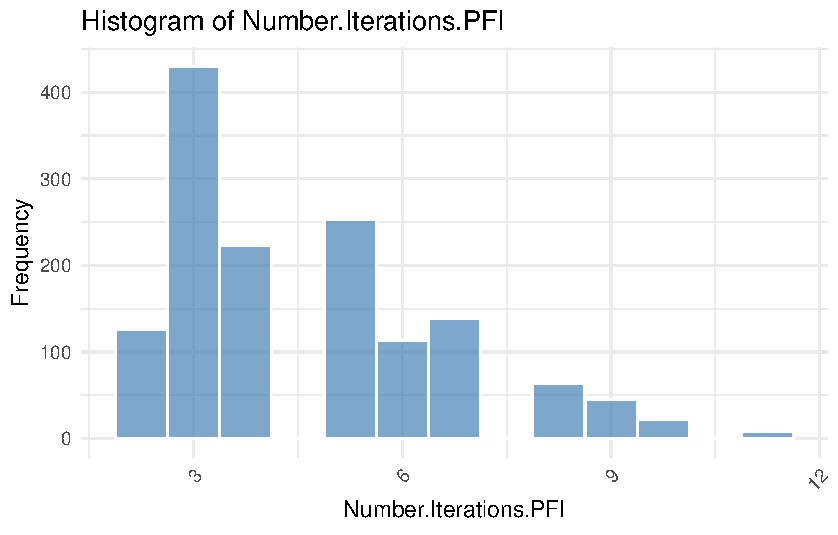
\includegraphics[width=\textwidth]{figures/histo_iter_pfi.pdf}
    \caption{Boxplot for number of iterations for PFI for JOB dataset. This shows that PFI takes a small number of iterations for our dataset, so we do not need to refactorize the basis matrix.}
    \label{fig:num_iter_boxplot_pfi_job}
\end{figure}


\begin{figure}[!htb]
    \centering
    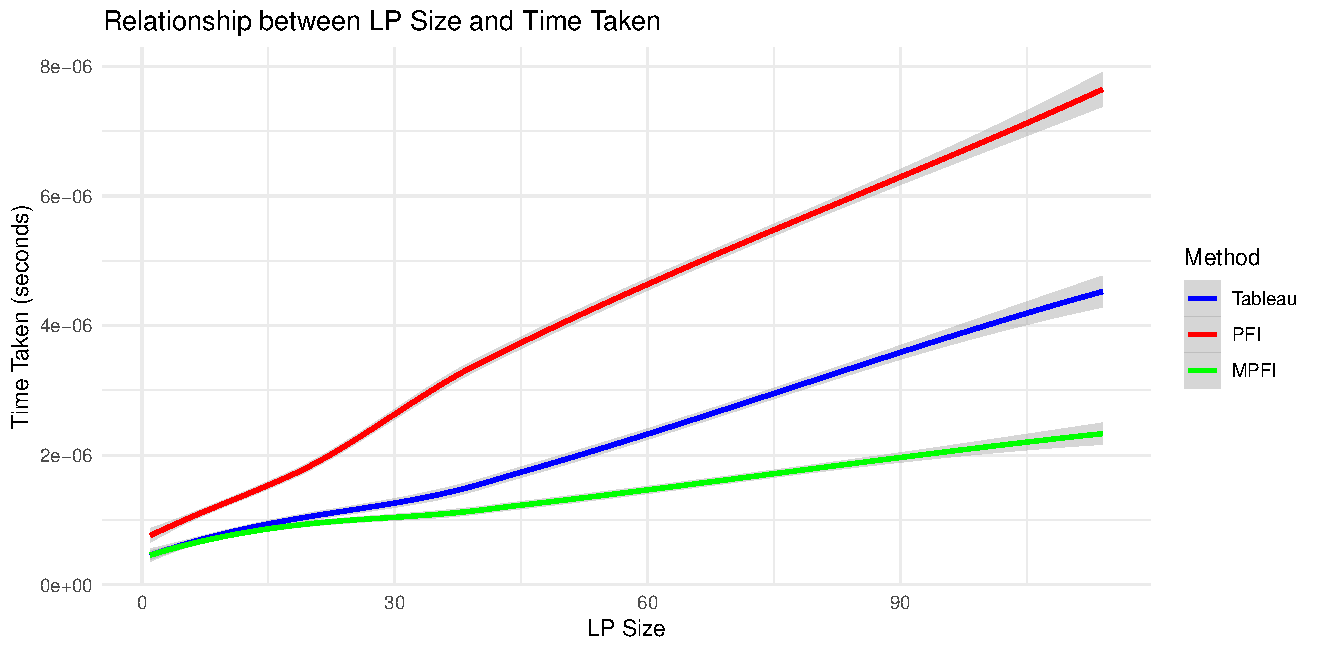
\includegraphics[width=\textwidth]{figures/job_methods_time.pdf}
    \caption{Relation between LP size and time for the 3 simplex solvers for JOB dataset.}
    \label{fig:lp_size_vs_time_job}
\end{figure}

\begin{figure}[!htb]
    \centering
    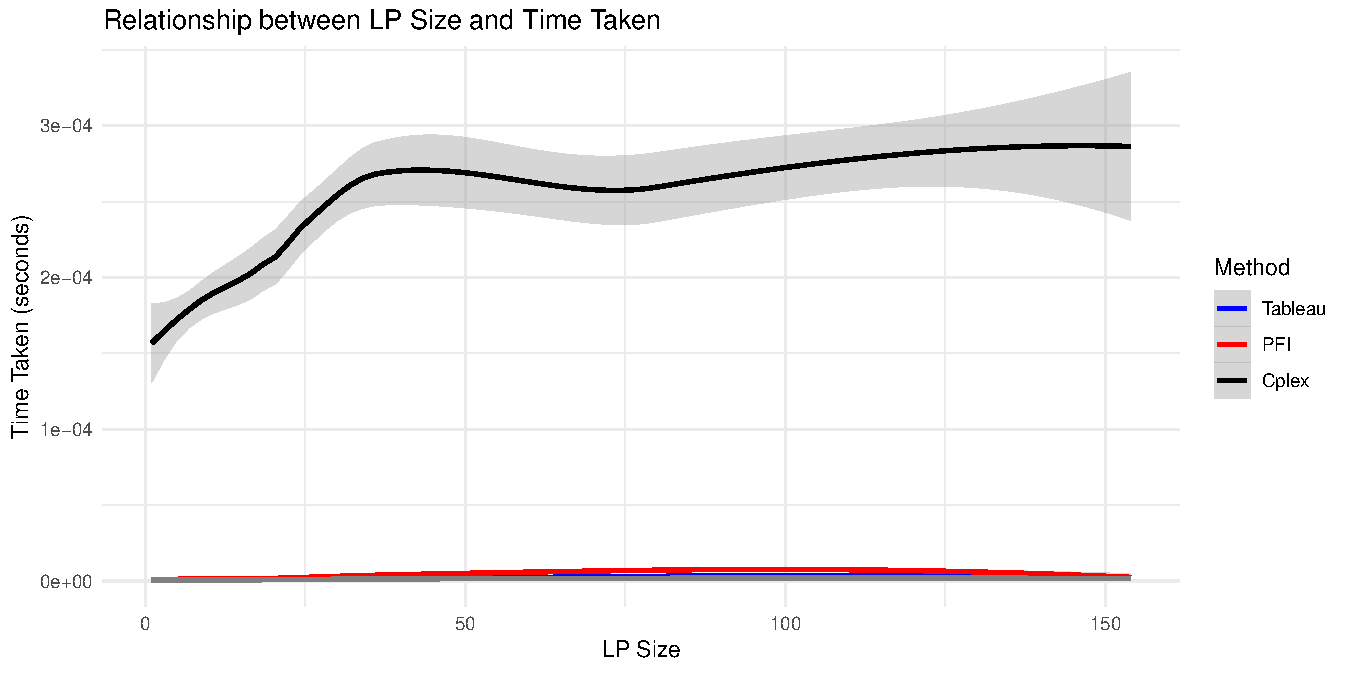
\includegraphics[width=\textwidth]{figures/cplex_vs_all_job.pdf}
    \caption{Relation between LP size and time for the 3 simplex solvers for JOB dataset and Cplex.}
    \label{fig:lp_size_vs_time_cplex_job}
\end{figure}

\begin{table}[!htb]
    \centering
    \caption{Statistics about JOB dataset, solution time is in microseconds.}
    \begin{tabular}{lrrrr}
        \toprule
        Variable                  & Min    & Median  & Mean    & Max     \\
        \midrule
        LP size                   & 1.00   & 18.00   & 26.46   & 114.00  \\
        Number of Rules           & 1.000  & 6.000   & 7.037   & 19.000  \\
        Number of Variables       & 1.00   & 3.00    & 3.07    & 6.00    \\
        Constraint Matrix Density & 0.3684 & 0.6667  & 0.6703  & 1.0000  \\
        Solution Time Cplex       & 96.08  & 193.60  & 204.18  & 651.84  \\
        Solution Time Tableau     & 0.160  & 0.970   & 1.301   & 11.060  \\
        Solution Time PFI         & 0.660  & 1.770   & 2.334   & 10.260  \\
        Solution time MPFI        & 0.1200 & 0.8900  & 0.9866  & 7.1800  \\
        Number Iterations Tableau & 2.000  & 4.000   & 4.829   & 14.000  \\
        Number Iterations PFI     & 2.000  & 4.000   & 4.621   & 11.000  \\
        Number Iterations MPFI    & 2.000  & 4.000   & 4.671   & 13.000  \\
        Optimal Value             & 0.3188 & 20.6702 & 21.8575 & 42.1804 \\
        \bottomrule
    \end{tabular}
    \label{table_job_stats}
\end{table}

\begin{table}[!htb]
    \centering
    \caption{Number of LPs or Queries Solved by Hour for the JOB dataset}
    \begin{tabular}{l|r}
        \toprule
        Method                     & Number of LPs/Hour \\
        \midrule
        Revised Simplex MPFU Umbra & 3,809,424,659          \\
        Tableau Simplex            & 2,870,945,324         \\
        Revised Simplex PFI        & 1,521,766,898         \\
        SciPy (method highs)       & 4,069,108             \\
        Cplex                      & 18,180,632            \\
        \bottomrule
    \end{tabular}
    \label{table_lps_hr_job}
\end{table}



\subsubsection{TPC-DS results}
In the Table \ref{stat_tpcds} are some important statistical findings following our
experiments with the TPC-DS dataset.
We collect the data and perform plotting and data summary using R scripts. The results can be
viewed in the Figures \ref{fig:num_iter_tpcds_mpfi}, \ref{fig:cplex_time_tpcds}, \ref{fig:methods_time_tpcds} and \ref{fig:num_iter_pfi_tpcds}.
\begin{table}[h]
    \centering
    \caption{Statistics about the TPC-DS dataset, the solution time is expressed in microseconds.}
    \begin{tabular}{lcccc}
        \toprule
        Variable                  & Min    & Median & Mean   & Max    \\
        \midrule
        LP size                   & 1.00   & 20.00  & 33.51  & 154.00 \\
        Number of Rules           & 1.00   & 6.00   & 7.88   & 22.00  \\
        Number of Variables       & 1.000  & 3.000  & 3.234  & 7.000  \\
        Constraint Matrix Density & 0.4365 & 0.8000 & 0.7415 & 1.0000 \\
        Solution Time Cplex       & 94.65  & 209.81 & 219.54 & 543.36 \\
        Solution Time Tableau     & 0.190  & 0.990  & 1.459  & 11.370 \\
        Solution Time PFI         & 0.730  & 1.980  & 2.965  & 32.540 \\
        Solution time MPFI        & 0.2700 & 0.9800 & 1.1139 & 7.7000 \\
        Number Iterations Tableau & 2.000  & 4.000  & 4.315  & 11.000 \\
        Number Iterations PFI     & 2.000  & 4.000  & 4.288  & 12.000 \\
        Number Iterations MPFI    & 2.000  & 4.000  & 4.228  & 12.000 \\
        Optimal Value             & 4.82   & 14.48  & 15.95  & 34.60  \\
        \bottomrule
    \end{tabular}
    \label{stat_tpcds}
\end{table}


\begin{figure}[!htb]
    \centering
    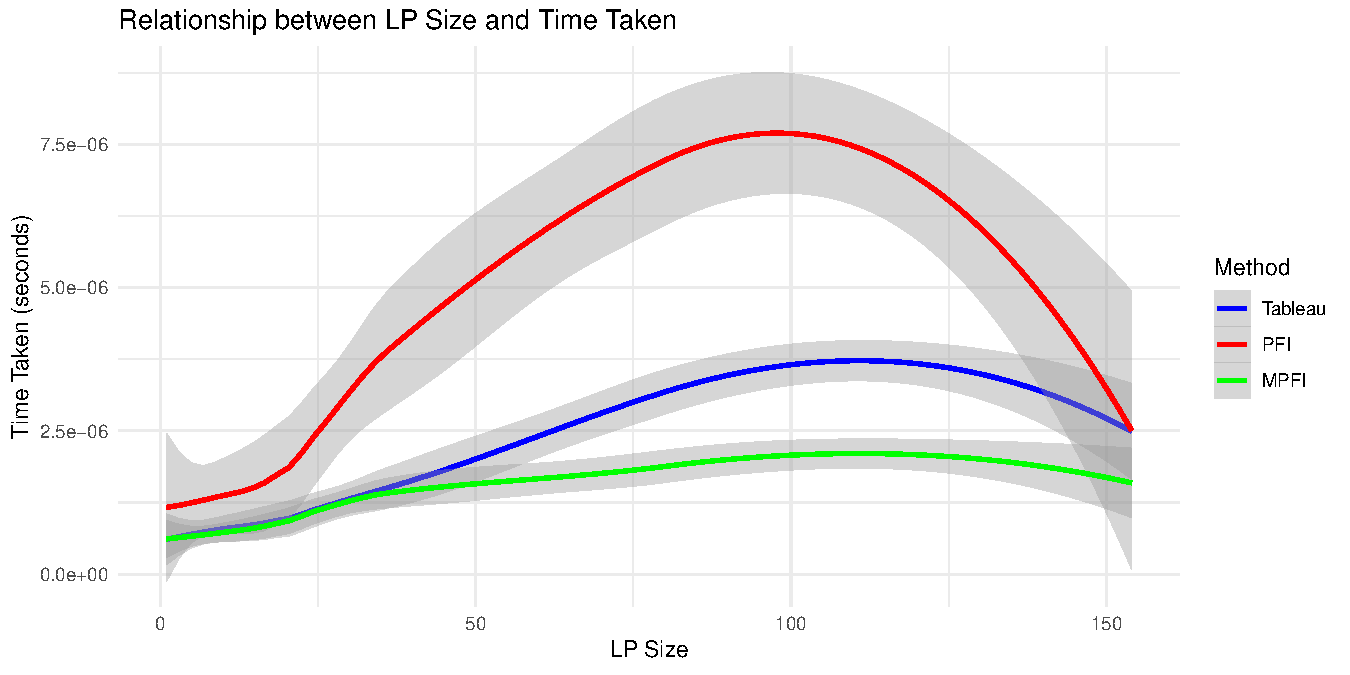
\includegraphics[width=\linewidth]{figures/methods_time_tpcds.pdf}
    \caption{Time profile comparison (Relationship between time and LP-size) of our 3 solvers solving the TPC-DS dataset}
    \label{fig:methods_time_tpcds}
\end{figure}

\begin{figure}[!htb]
    \centering
    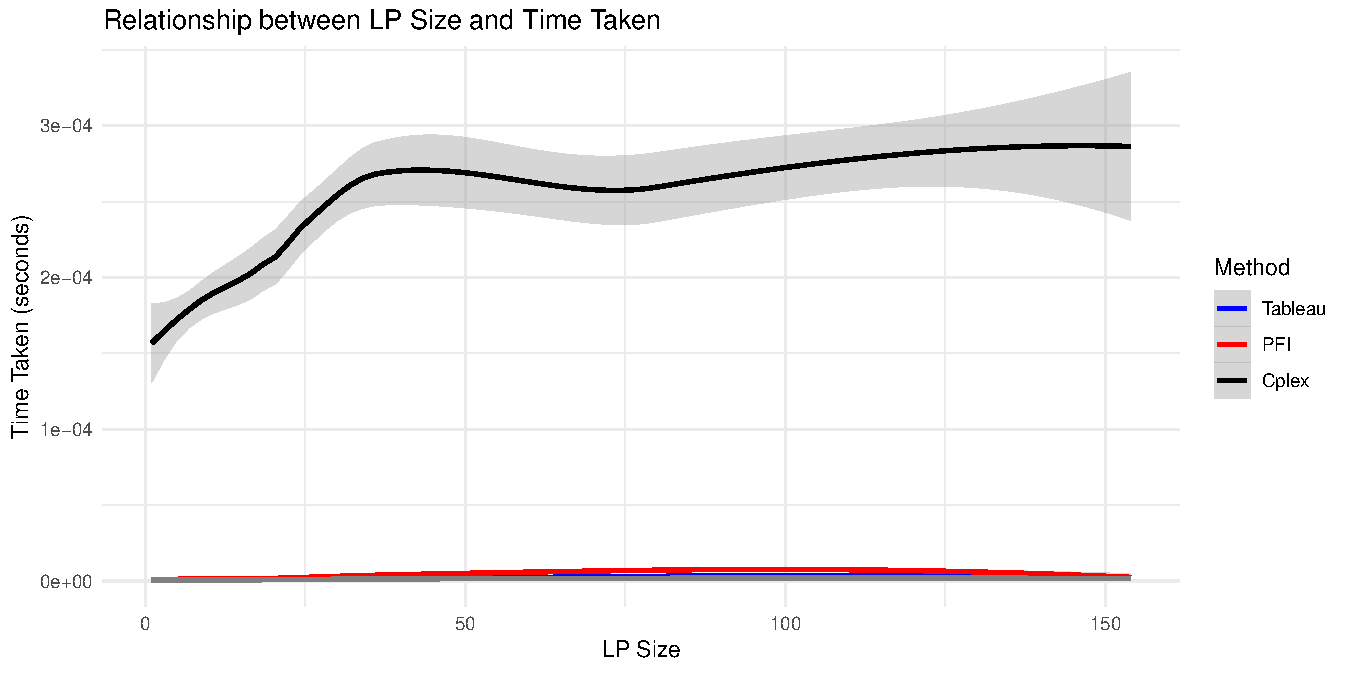
\includegraphics[width=\linewidth]{figures/cplex_vs_all_tpcds.pdf}
    \caption{Time profile comparison (Relationship between time and LP-size) of our 3 solvers and Cplex solving the TPC-DS dataset}
    \label{fig:cplex_time_tpcds}
\end{figure}

\begin{figure}[!htb]
    \centering
    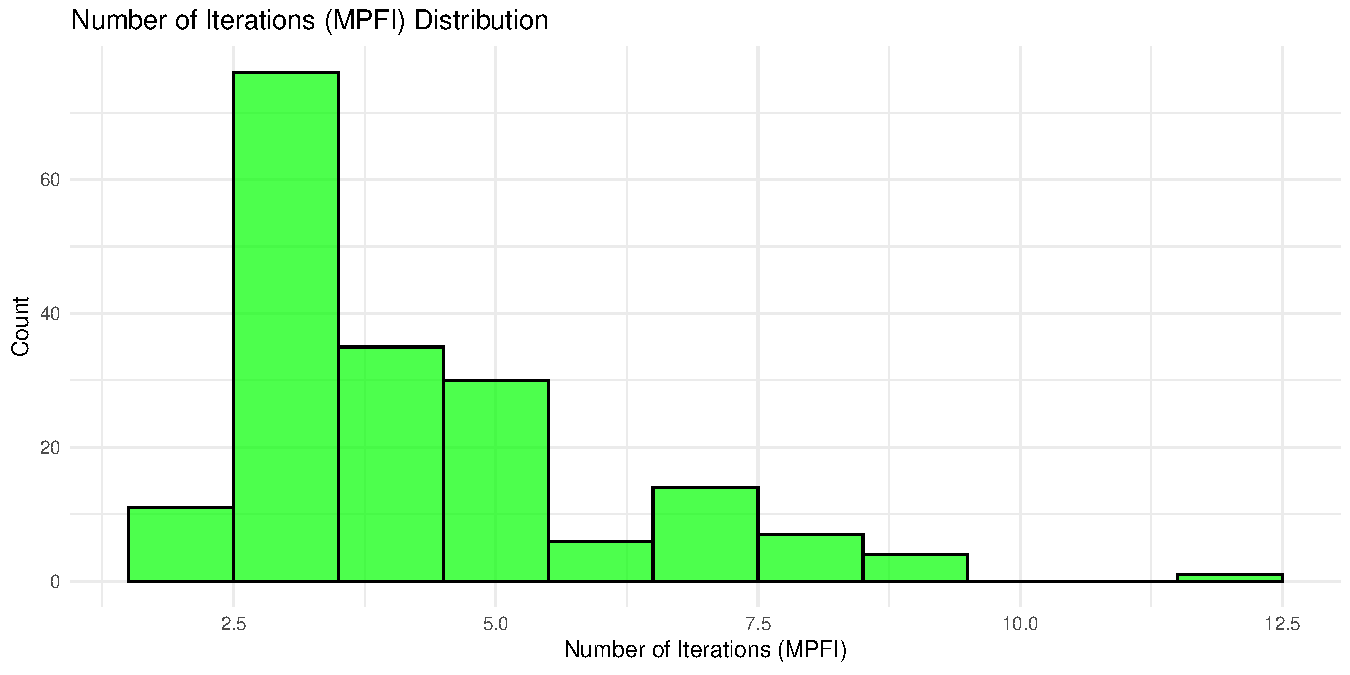
\includegraphics[width=\linewidth]{figures/num_iter_tpcds_mpfi.pdf}
    \caption{Histogram for number of iterations for MPFI for TPC-DS dataset}
    \label{fig:num_iter_tpcds_mpfi}
\end{figure}

\begin{figure}[!htb]
    \centering
    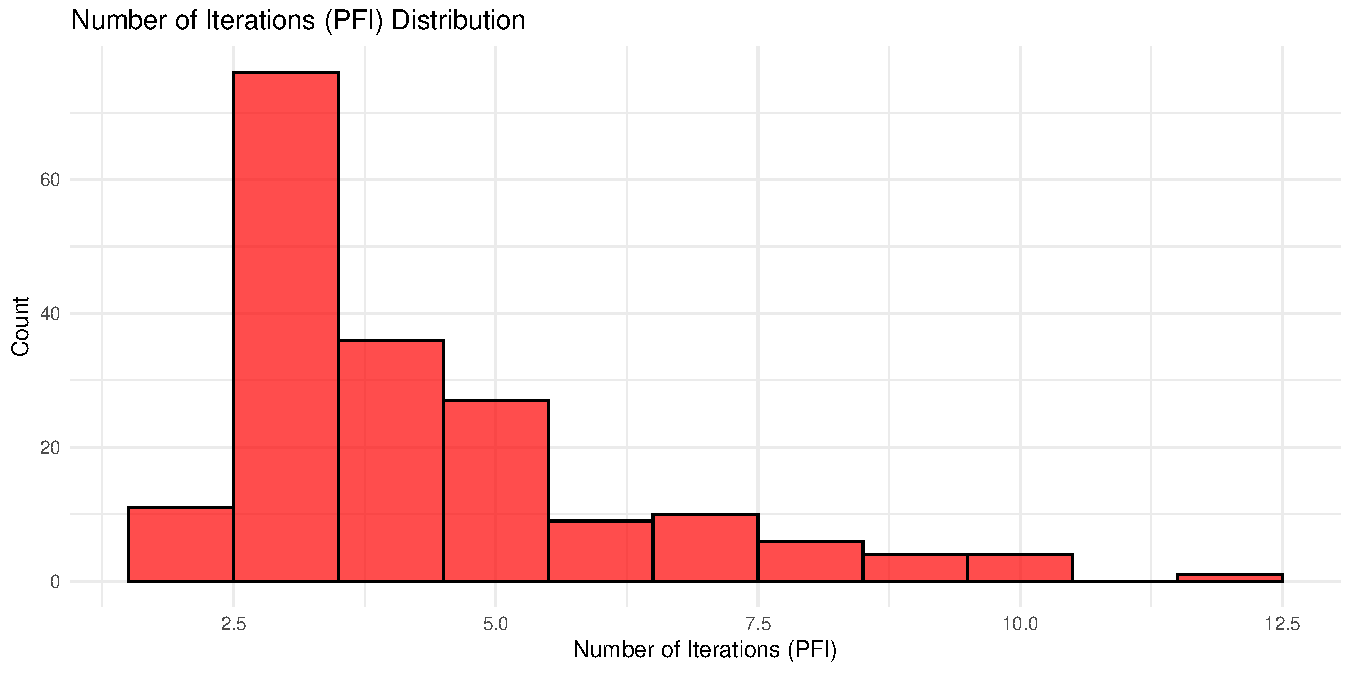
\includegraphics[width=\linewidth]{figures/num_iter_pfi_tpcds.pdf}
    \caption{Histogram for number of iterations for PFI for TPC-DS dataset}
    \label{fig:num_iter_pfi_tpcds}
\end{figure}


\subsubsection{TPC-H results}
In the Tables \ref{stat_tpch} and \ref{table_lps_hr_tpch} are some important statistical finds following our
experiments with the TPC-H dataset.
We collect the data and perform plotting and data summary using R scripts. The results can be
viewed in the Figures \ref{fig:cplex_time_tpch}, \ref{fig:methods_time_tpch} and \ref{fig:speedup_tpch}.

\begin{figure}[!htb]
    \centering
    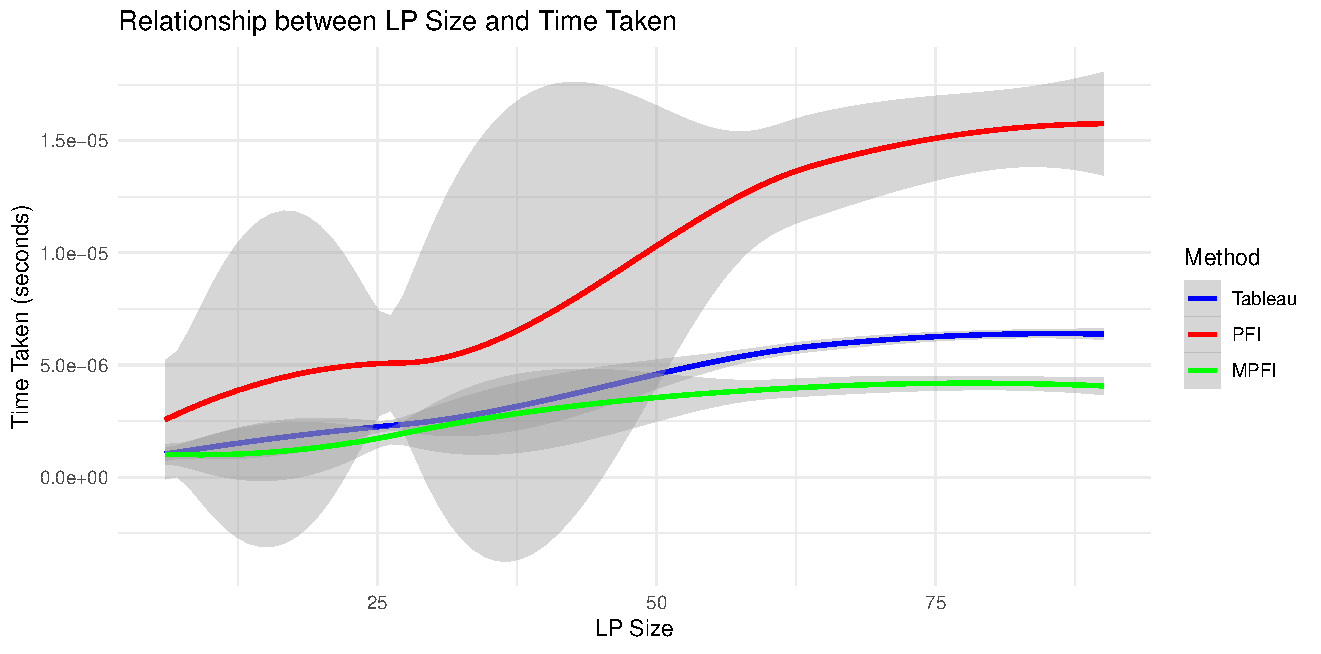
\includegraphics[width=\linewidth]{figures/methods_time_tpch.pdf}
    \caption{Time profile comparison (Relationship between time and LP-size) of our 3 solvers solving the TPC-H dataset }
    \label{fig:methods_time_tpch}
\end{figure}
\begin{figure}[!htb]
    \centering
    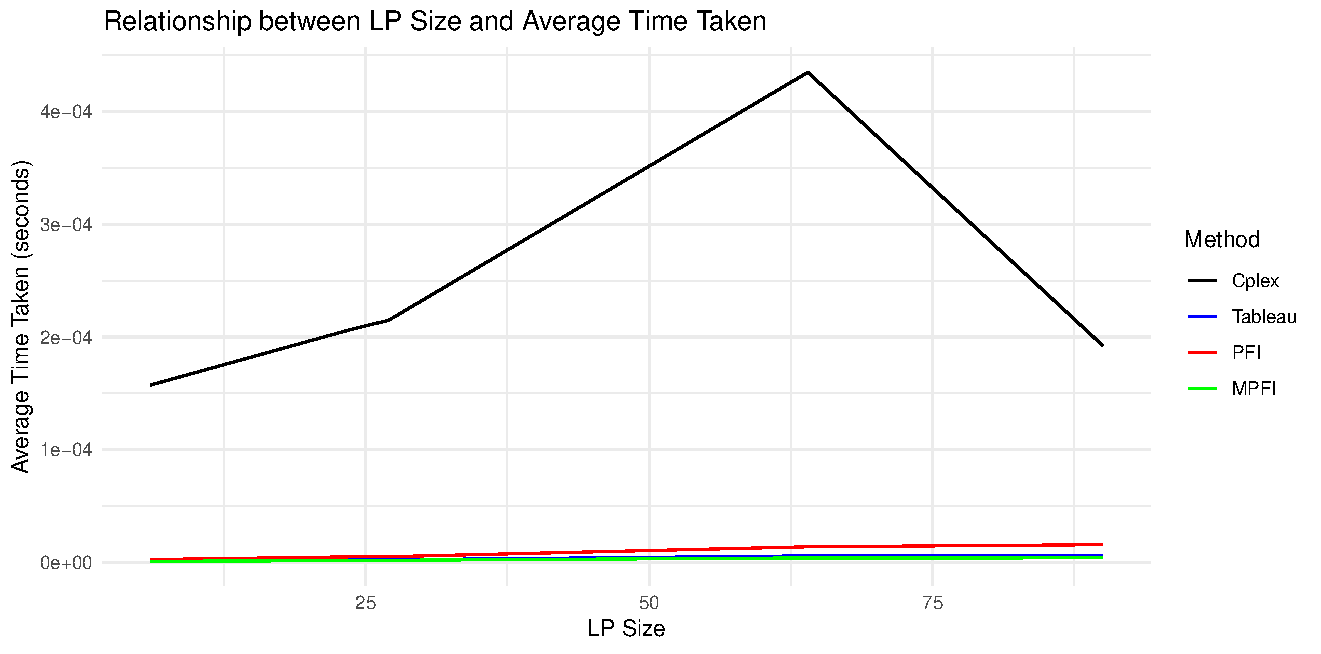
\includegraphics[width=\linewidth]{figures/cplex_vs_all_tpch.pdf}
    \caption{Time profile comparison (Relationship between time and LP-size) of our 3 solvers and Cplex solving the TPC-H dataset}
    \label{fig:cplex_time_tpch}
\end{figure}
\begin{figure}[!htb]
    \centering
    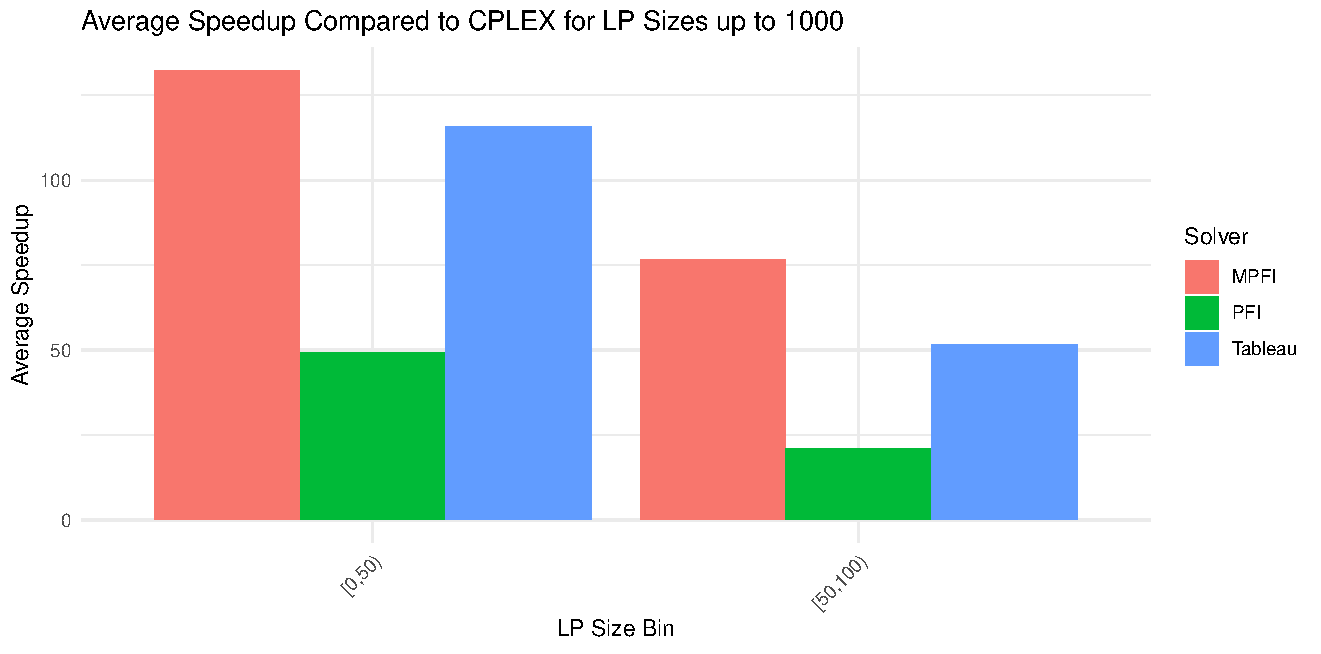
\includegraphics[width=\linewidth]{figures/speedup_tpch.pdf}
    \caption{Speedup of our 3 solvers solving the TPC-H dataset compared to Cplex. }
    \label{fig:speedup_tpch}
\end{figure}


\begin{table}[!htb]
    \centering
    \caption{Number of LPs Solved by Hour for the TPC-H dataset}
    \begin{tabular}{l|r}
        \toprule
        Method                     & Number of LPs/Hour \\
        \midrule
        Revised Simplex MPFU Umbra & 1,295,255,228      \\
        Tableau Simplex            & 909,090,909        \\
        Revised Simplex PFI        & 379,997,361        \\
        Cplex                      & 8,042,340          \\
        \bottomrule
    \end{tabular}
    \label{table_lps_hr_tpch}
\end{table}
\begin{table}
    \centering
    \caption{Statistics about the TPC-H dataset, the solution time is expressed in microseconds.}
    \begin{tabular}{lcccc}
        \toprule
                                           & \textbf{Min.} & \textbf{Median} & \textbf{Mean} & \textbf{Max.} \\
        \midrule
        \textbf{Number of Rules}           & 3.00          & 12.50           & 11.75         & 18.00         \\
        \textbf{Number of Variables}       & 2.000         & 3.500           & 3.562         & 5.000         \\
        \textbf{Constraint Matrix Density} & 0.4111        & 0.6146          & 0.6132        & 0.8333        \\
        \textbf{Solution Time Cplex}       & 149.2         & 200.5           & 252.6         & 1059.3        \\
        \textbf{Solution Time Tableau}     & 1.010         & 4.230           & 3.960         & 6.510         \\
        \textbf{Solution Time PFI}         & 2.540         & 7.970           & 9.474         & 19.050        \\
        \textbf{Solution time MPFI}        & 1.010         & 2.740           & 2.779         & 4.700         \\
        \textbf{Number Iterations Tableau} & 3.0           & 5.5             & 5.0           & 7.0           \\
        \textbf{Number Iterations PFI}     & 3.00          & 5.00            & 5.50          & 8.00          \\
        \textbf{Optimal Value}             & 14.44         & 20.73           & 19.69         & 22.77         \\
        \bottomrule
    \end{tabular}
    \label{stat_tpch}
\end{table}
%------------------------------------------------------------------------
\subsection{Results on randomly generated LPs}
We also test our solvers alongside Cplex, on packing LPs generated randomly.

We use a Python script as a generator for packing linear programming (LP) problems.
It creates LP problem instances
based on the specified number of rules and variables.
For each rule, a random number of entries, ranging from 1 to
the total number of variables, is determined.
For every entry in a rule, a unique column number is randomly selected from
the available variables, ensuring that the same column is not used more than once for
the same rule. A random coefficient, between 0.1 and 1.0, is then assigned to
this column. The entire LP problem is represented as a space-separated string,
where the first entry denotes the number of rules, followed by the number of
entries for each rule, and then the column-coefficient pairs.
The main part of
the script generates a series of such LP problems, incrementally increasing the
number of rules and variables for each problem, and write them in a text file.
This is how we get our randomly generated packing LPs with increasing sizes in the same format
as the query datasets.

We run our solvers, and also Cplex on this dataset, which provides us with numerical results
in the figures: \ref{fig:time_vs_size_random}, \ref{fig:lps_per_hour_random}, \ref{fig:size_time_random_large},
\ref{fig:speedup_cplex_less_1000.pdf}, and \ref{fig:speedup_cplex_random.pdf}.

We want to
explore those results to investigate how these solvers scale, and if the speedup
they provide is still substantial at larger LPs.


\begin{figure}[!htb]
    \centering
    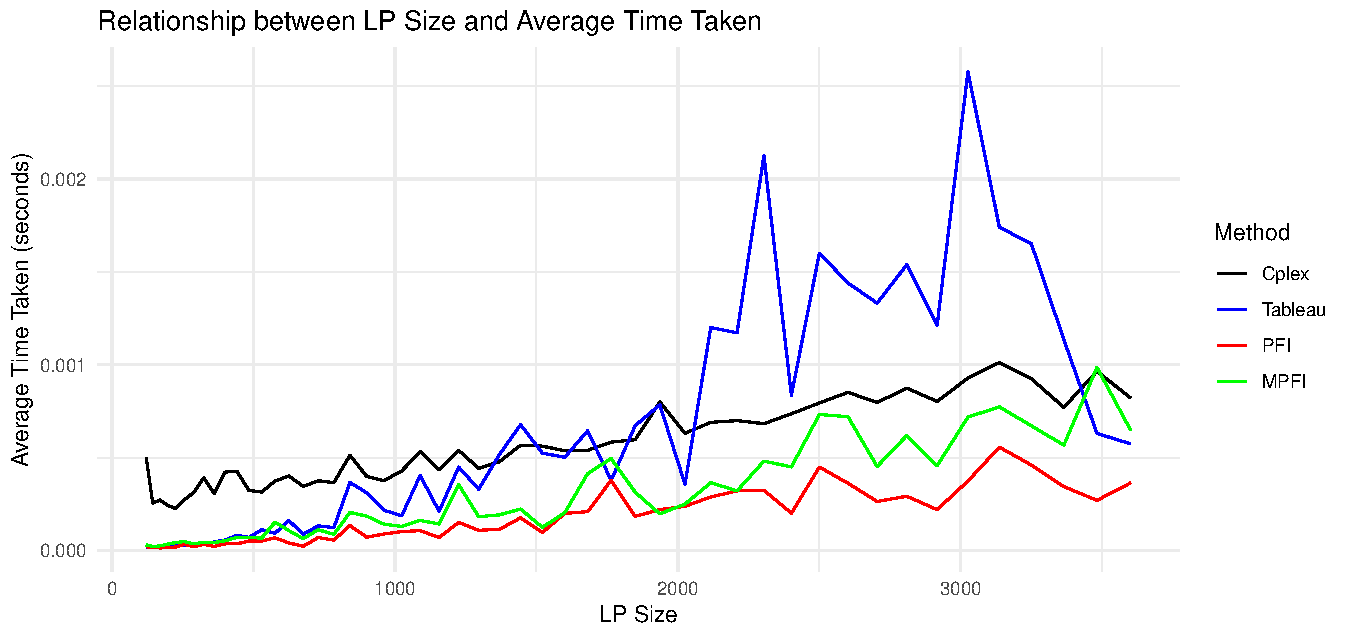
\includegraphics[width=0.8\textwidth]{figures/time_vs_size_random.pdf}
    \caption{Relation between LP size and time for the 3 simplex solvers and Cplex for randomly generated
        dataset with increasing LP size.}
    \label{fig:time_vs_size_random}
\end{figure}


\begin{table}[!htb]
    \centering
    \caption{Number of LPs Solved by Hour for the randomly generated dataset}
    \begin{tabular}{l|r}
        \toprule
        Method                     & Number of LPs \\
        \midrule
        Revised Simplex MPFU Umbra & 13,520,349    \\
        Tableau Simplex            & 6,963,530     \\
        Revised Simplex PFI        & 24,352,331    \\
        Cplex                      & 6,666,083     \\
        \bottomrule
    \end{tabular}
    \label{fig:lps_per_hour_random}
\end{table}

We get the time profile in Figure \ref{fig:time_vs_size_random}.
We want to see the further evolution of this time profile, so we increase the number of generated LPs
and explore larger LPs, see Figure \ref{fig:size_time_random_large}.

\begin{figure}[!htb]
    \centering
    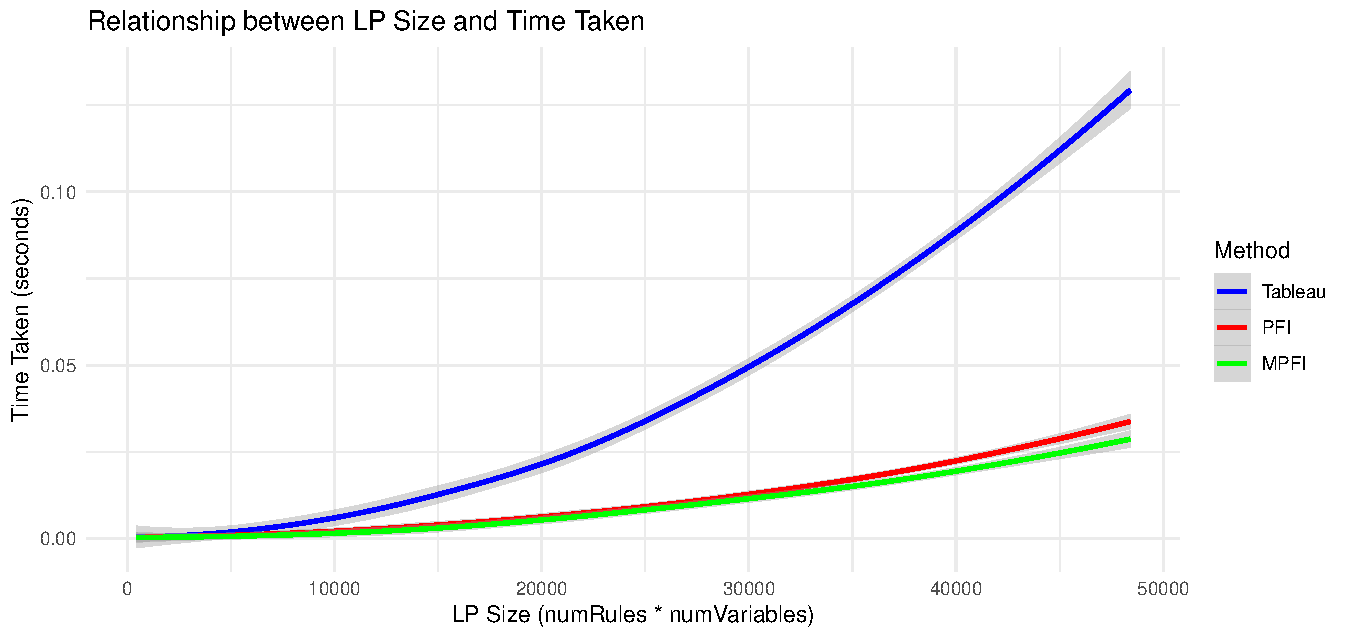
\includegraphics[width=\linewidth]{figures/size_time_random_large.pdf}
    \caption{Relation between LP size and time for the 3 simplex solvers for the randomly generated
        dataset with increasing LP size ranging up to 220 rules and 220 variables.}
    \label{fig:size_time_random_large}
\end{figure}

\begin{figure}[p]
    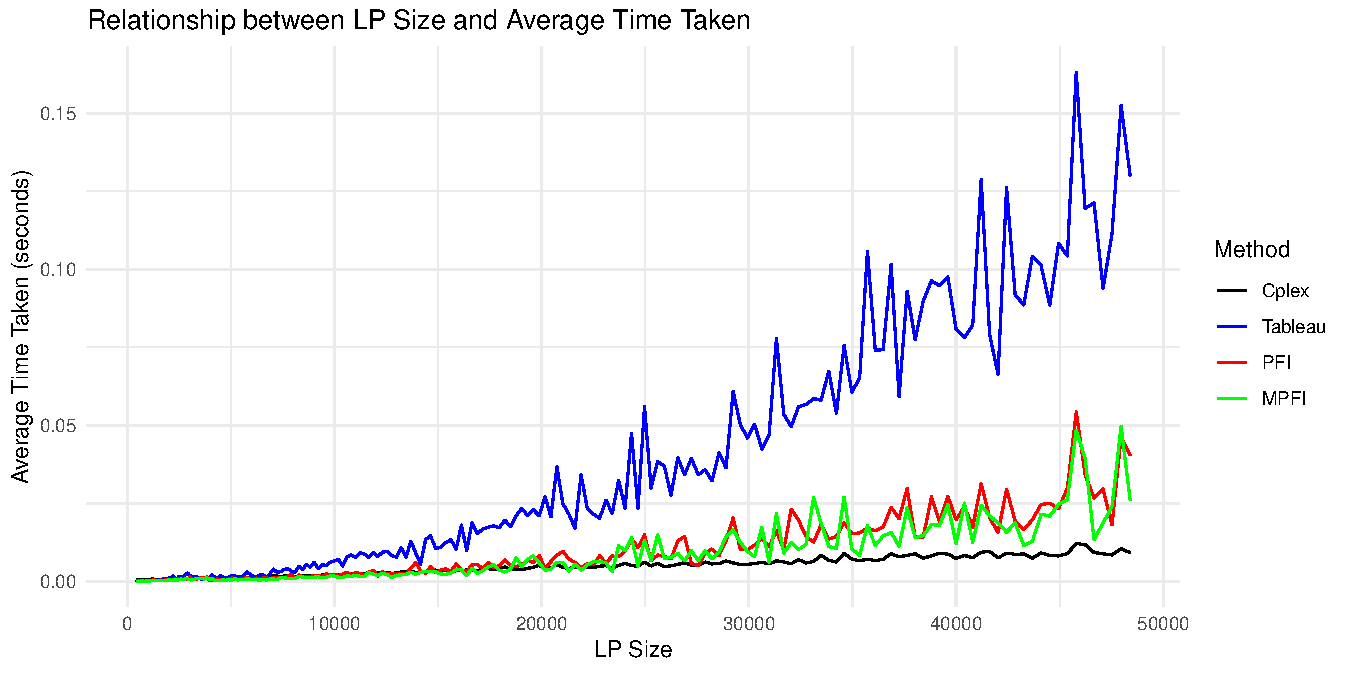
\includegraphics[width=0.8\paperwidth, height=\paperheight, keepaspectratio]{figures/cplex_vs_all_random_large.pdf}
    \caption{Relation between LP size and time for the 3 simplex solvers with CPLEX randomly generated
        dataset with increasing LP size ranging up to 220 rules and 220 variables.}
    \label{cplex_vs_all_random_large}
\end{figure}

\begin{figure}[!htb]
    \centering
    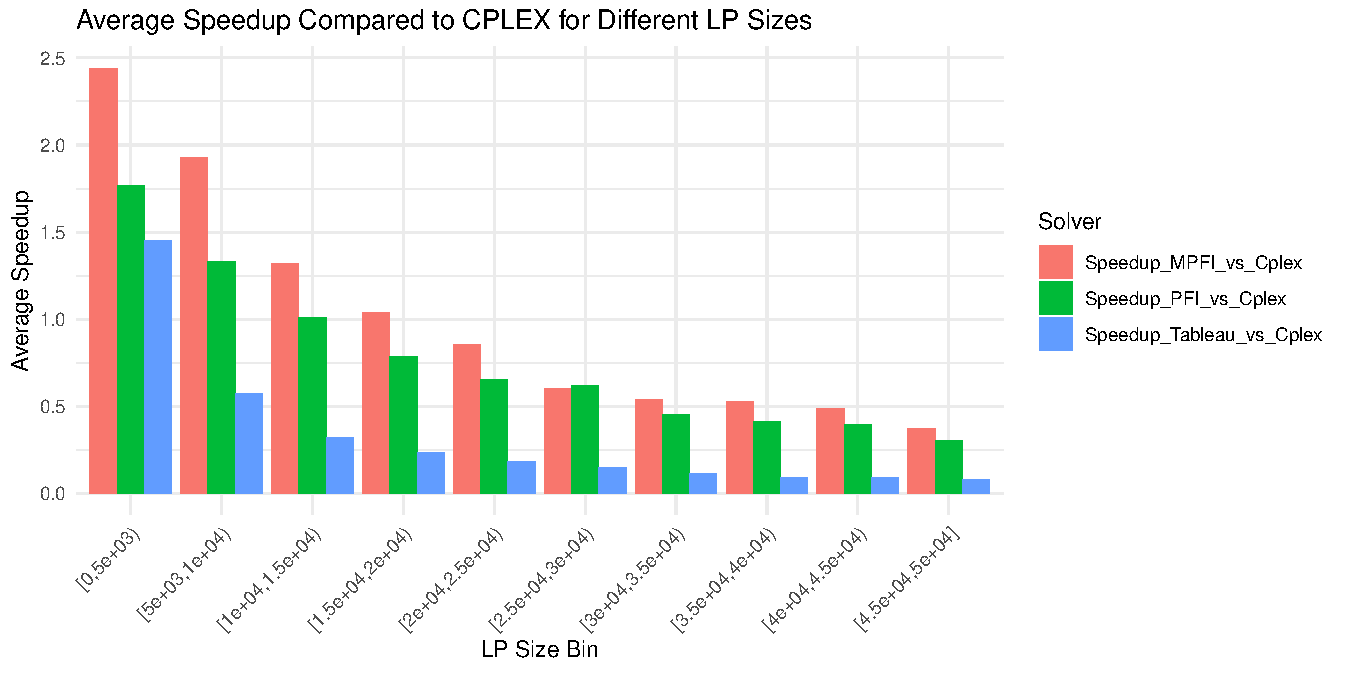
\includegraphics[width=\linewidth]{figures/speedup_vs_cplex_random_200.pdf}
    \caption{Speedup of the three solvers (how many times faster they are) compared to CPLEX for
        the randomly generated dataset for increasing LP size}
    \label{fig:speedup_cplex_random.pdf}
\end{figure}

\begin{figure}[!htb]
    \centering
    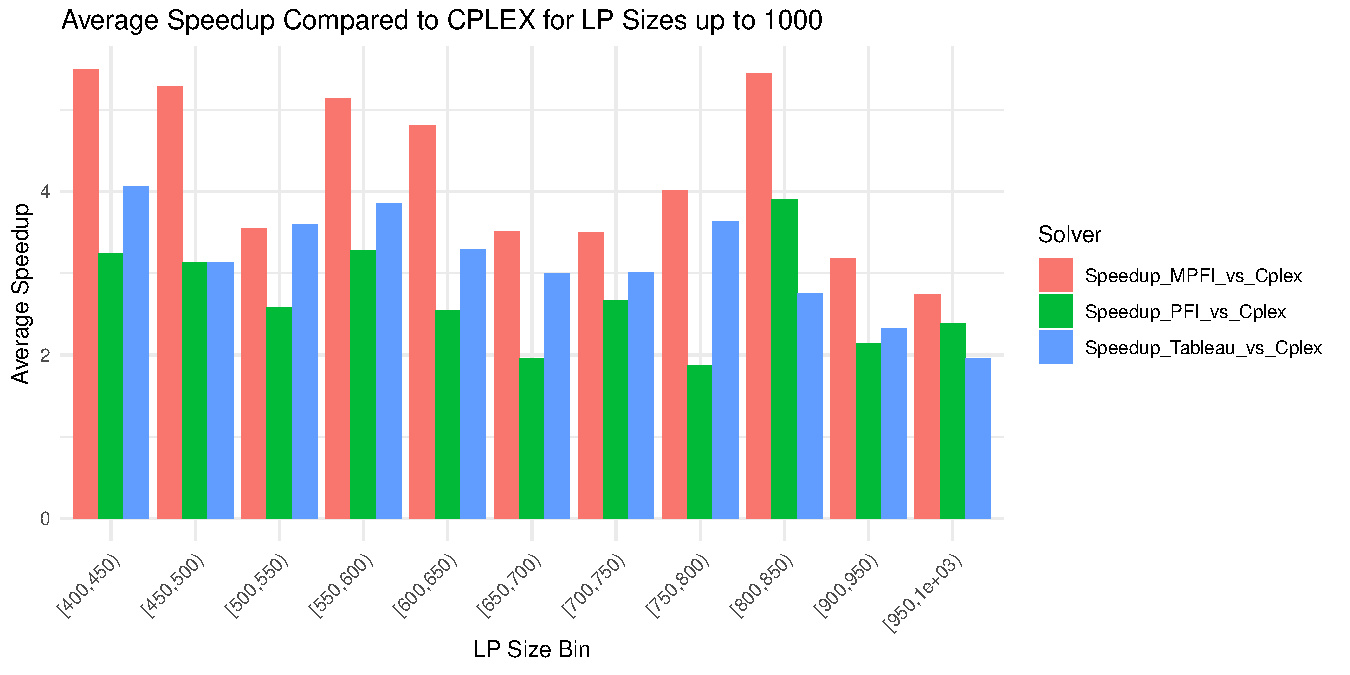
\includegraphics[width=\linewidth]{figures/speedup_cplex_less_1000.pdf}
    \caption{Speedup of the three solvers (how many times faster they are) compared to CPLEX for
        the randomly generated dataset for the LP size up to 1000}
    \label{fig:speedup_cplex_less_1000.pdf}
\end{figure}

%------------------------------------------------------------------------


